\section{Pointer Tagging}
\label{sec:preliminaries:pointertagging}

Pointer Tagging is a low-level programming technique that uses the spare low bits in a pointer to encode additional information. Using the Pointer tagging technique, pointer value (initially a memory address before tagging) can hold extra information about the point-to heap object or can be used as a meta-data to further describe the usage of the pointer data. Pointer tagging is mainly enabled because of the way heap objects are situated and accessed on modern computer architectures.


\myworries{metaphorically}

\subsection{Data Structure Alignment}
\label{sec:preliminaries:data_alignment}
Data alignment (also referred to as data structure padding) is a way in which heap objects are arranged and accessed by the CPU. CPUs in modern computer architecture (say 64-bit architecture) read data from and write data to memory more efficiently when data is aligned.  \\

On an abstract level, computer memory can be seen as an array of words or bytes, each with its own address. Unlike bytes, the term word has ambiguate meaning. In the context of this work, we are targeting the generic term in the context of CPU architecture. That is, a "processor word" refers to the size of a processor register or memory address register. The term word also refers to the size of CPU instruction, or the size of a pointer depending on the exact CPU architecture. For example, in a 64-bit architecture, the word size (also pointer size) is 64 bits = 8 bytes.\todo{Figure need to be added} \\

Generally, when a source program is executed, it is loaded into memory and put into a process $p$ for execution. All data objects in the program are mapped at certain point in time (during compilation or execution) to a physical memory address [ref: operating system concept]. Let us suppose we have the following snippet written in C language: \\

\begin{verbatim}
bool *b = new bool(true); // x = x21DE
int* a = new int(123);  // a = x21E6
char* c = new char(‘A’);  // c = x21EE
\end{verbatim}

According to C language specification, the size of integer value in memory is 4 bytes and size of char value is 1 byte [C spec]. When we execute the previously mentioned statements, however, the compiler (or linker) books 8 bytes of memory to hold the integer value and not 4 bytes as expected. The reason is that, the compiler adds padding to the heap objects in order to align them in memory. The same applies to the character value, as shown in figure 1 (on my notebook).  \\

Why data alignment? The CPU can access the memory only in word-sized chunks. So if our data always starts at a word it can be fetched efficiently. If it were to start somewhere in the middle of a word, the CPU will need to wait two or more memory cycles to fetch data from or write data to memory causing an increase in the CPU stall period which results in a significant performance overhead. \\


many modern compilers implementations handle data alignment in memory automatically, example includes C, C++, Rust, C\# compilers.

\begin{figure}
	\centering
	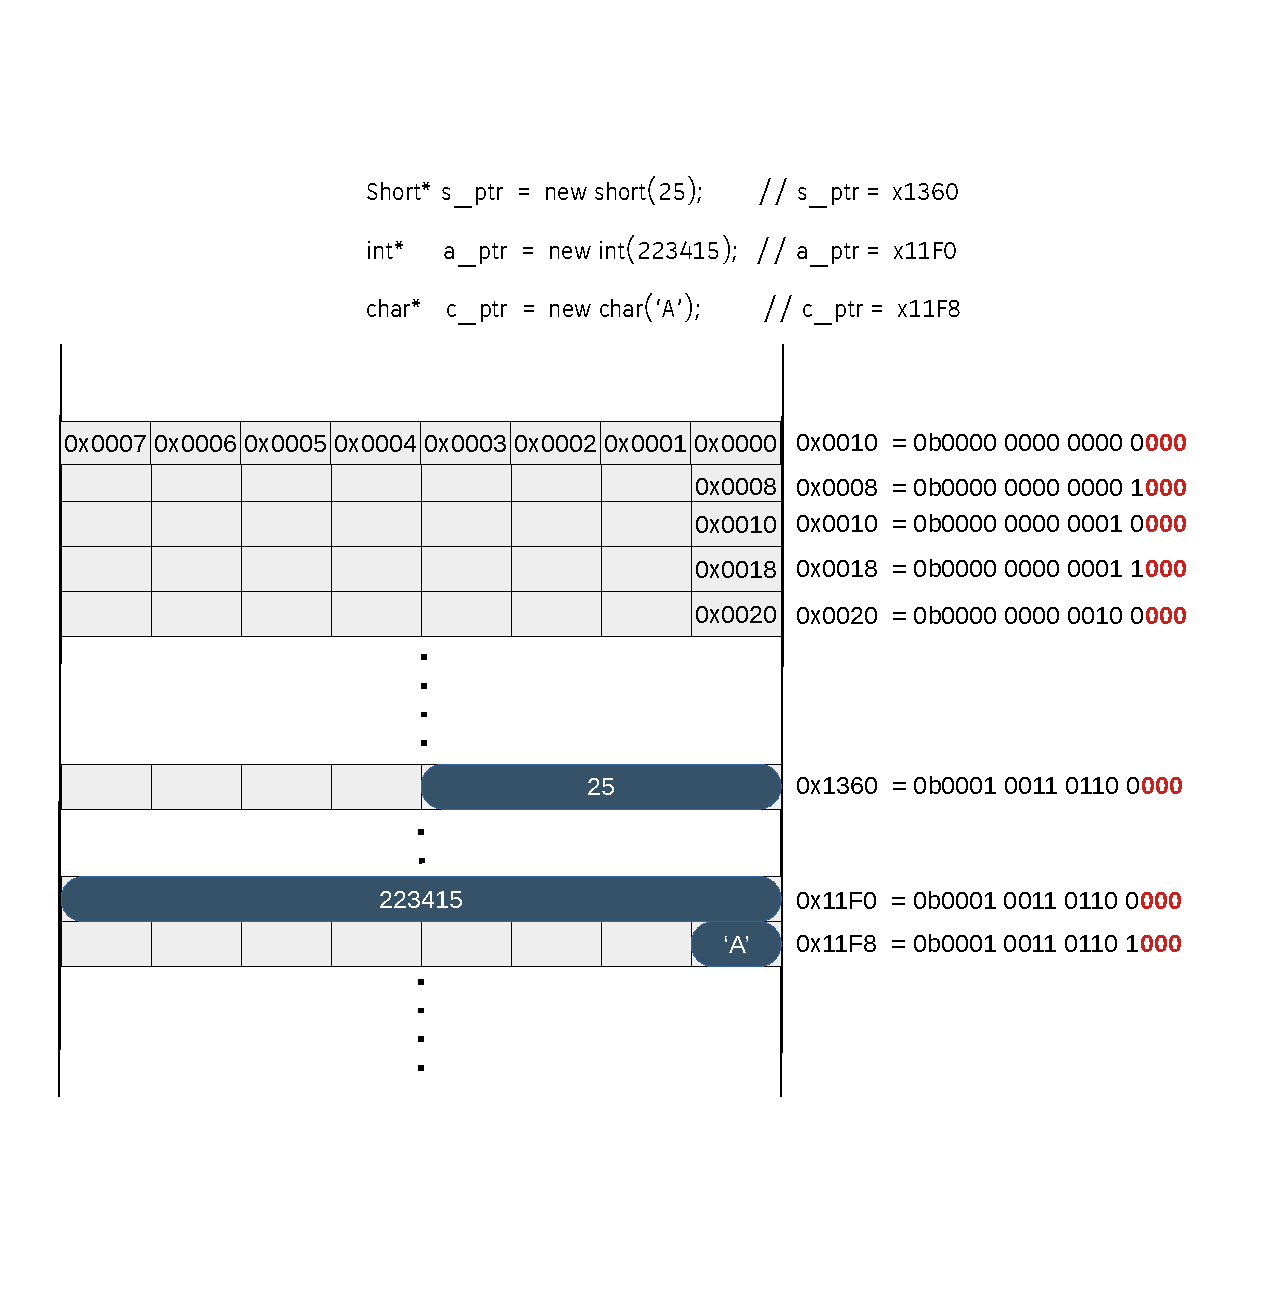
\includegraphics[scale=0.8]{figures/chapter2/memorylayout}
	\caption{Trie representation of the tensor $T_g$ that depicts the RDF graph $g$ in  Table \ref{tab:ma_tensor}. A slice $T_g[3, :, :]$ by the first dimension with 3 is shown in the red (inner) box.}
	\label{fig:data_aligntment}
\end{figure}

\subsection{Tagged Pointers}
Some high-level programming languages, for example C++, offer developers a tool set to work with memory. Using such tool set, developers have access to low level memory abstraction. The main building block that enables memory management is the \textbf{pointer data type} and its ecosystem. A variable of type pointer holds a memory address of an object stored in the heap. Due to data alignment (cf. \ref{sec:data_alignment}), the memory address of any object in the heap memory is always $\alpha\cdot w$ where $w=8$ (the word size). This implies all addresses held as a pointer value are multiple of 8. A pointer thus can be 8, 16, 24, 109144, etc. But it can not be 7 or 13. \\

\begin{figure}
	\centering
	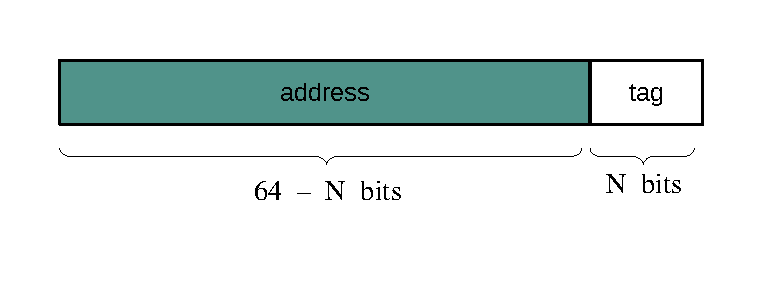
\includegraphics[scale=1]{figures/chapter2/pointervalue}
	\caption{Trie representation of the tensor $T_g$ that depicts the RDF graph $g$ in  Table \ref{tab:ma_tensor}. A slice $T_g[3, :, :]$ by the first dimension with 3 is shown in the red (inner) box.}
	\label{fig:tagged_pointer}
\end{figure}


Speaking in binary, example of pointer values are 0b1000 (=8), 0b10000 (=16), 0b11000 (=24), 0b11010101001011000 (=109144). The lower three bits, also called the least significant bits (LSBs), are always zero. So those three bits are basically free to use. We can use them to store a \textbf{tag}, which is an integer between 0 (0b000) and 7 (0b111).  \\ 

Pointer tagging technique allows a dynamic representation of the value based on the tag. Thus, the actual bits payload of the pointer could represents a memory address for some time during the process execution but can later express the binary representation of a \texttt{char} value for example, depending on the execution context and after a change in the tag value during run-time. \\

An approach to implement a tagged pointer is to develop a wrapper object around a pointer type variable. The wrapper can be equipped with adequate behaviours that govern the tag/ payload manipulation and retrieval. An example of pointer tagging implementation can be seen in listing (\todo{Add the listing}) \\
 
Pointer tagging can be applied in many use cases. In my work, there are a couple of use cases where pointer tagging served perfectly the purpose. Namely: storing integers in pointers and Dynamic de-referencing of void pointers (\texttt{void*}).\todo{Need to check this} 					

\subsection{Tagged Pointer Implementation}

\myworries{Tagged pointers technique doesn't compromise address space/ but does affect memory safty}

\myworries{Doesn't add extra overhead of extra space utilization	}



\paragraph{Integer Tagged Pointer}

\paragraph{Type Tagged Pointer} \todo{Keep it for the time being}
Figure

\clearpage